\chapter{Introduction} 
\label{Introduction} % la etiqueta para referencias

% 1. Por qué comunicaciones ópticas?
% 2. Haces Laguerre-Gauss.
% 3. OAM.
% 4. ¿Qué es cancelación de haces?
% 5. Turbulencia Atmosférica.
% 6. Motivación.
%\enlargethispage{-0.2cm} %Para que quepa bien el pie de página.
We are living in the information era. Society has radically changed on a global scale since the popularization of internet in the 1990's, and even more so during these challenging times, where the global pandemic crisis has reinforced telecommunications as a backbone of modern civilization. The acquired importance that this area has in so many lives and businesses right now can be reason enough to justify the funding and research to enhance the current system's speed, safety and privacy. On this aspect, optical communications have rose recently for the last thirty years, as it is the case of optical fiber. A little history shows as that since the discovery of light's refractive properties in 1840, followed by the conception of the idea of fiber optics during the first half of the XX century, research and prototypes' developments during the second half of the same century, and until the first commercial implementation, popularization and widespread infrastructure during the 2000's (and still ongoing), there was a time span of over 150 years. A similar scenario is disguised in the recent development of free-space optics (FSO). In 1992, Les Allen et al. published a paper that unveiled that laser light can carry orbital angular momentum (OAM) several times larger than the already known spin angular momentum (SAM), and that it could be readily realizable in a laboratory \cite{Allen_OAM:1992}. 

Another important thing that this paper showed was that these so-called \textit{OAM beams} could serve as an orthogonal base to simultaneously transfer information on a same physical channel. Several other papers \cite{Ren:13} \cite{Gibson:04} \cite{Funes:17} have suggested that it is possible to multiplex OAM-modulated beams to enhance the capacity and spectral efficiency of an FSO based on the orthogonality of these symbols. Each symbol possesses a different topological charge, denoted by the symbol $\ell$, that allows for overlapping beams to be multiplexed, identified and demultiplexed with minimal crosstalk.

However, the great disadvantage that FSO systems must overcome (and that optical fiber does not) is atmospheric turbulence. This is a physical phenomenon caused by random variations in atmospheric temperature and pressure that result in density changes within the same volume \cite{Field_Guide_to_Atmospheric_Optics}. These density changes, in turn, result in variations in the medium's refractive index, absorption and dispersion in the beam's intensity and phase distortions on the same beam that can deform it \cite{Rodenburg:12}. Because atmospheric turbulence can distort beams, it can later interfere in the identification process that allows for demultiplexation in the receiver's interface, and therefore, wrongful demodulation.

Nevertheless, atmospheric turbulence is not the only way that an OAM beam can be distorted. Most setups used to send OAM beams in FSO require telescopes to restrain their natural radial size growth along propagation. There are two types of telescopes that present their own advantages and obstacles that are commonly used: On one hand, there are refractive telescopes, whose aperture size is restrained by the weight of the lens itself (it could collapse under its own weight if it is too large) and the lens' imperfections, which can distort light passing through it, specially on non-astronomical distances. On the other hand, Schmidt-Cassegrain telescopes can have larger apertures because at the center of it there is an obstruction, where a mirror redirects incoming light towards the eyepiece. Withal, while the central obstruction may not be meaningful in astronomical distances, at shorter ones it can cause phase distortions on beams passing through them.

\begin{figure}[htbp]
    \centering
    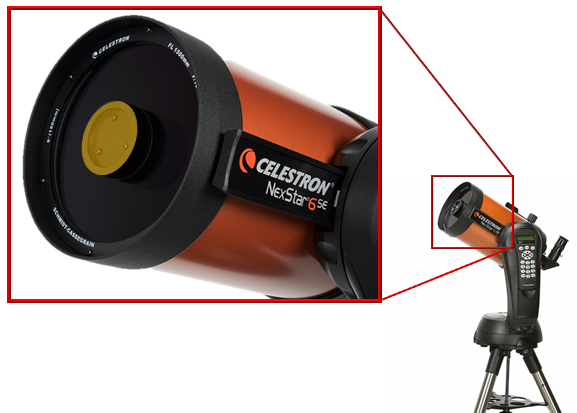
\includegraphics[width=9cm]{images/c03/Cassegrain-Obstruction.png}
    \caption{A Schmidt-Cassegrain telescope with its central obstruction highlighted in light yellow \cite{Schmidt-Cassegrain_Pics}.}
    \label{fig:intro-schmidt-cassegrain}
\end{figure}

At first, it may not seem like central obstruction could be harmful to OAM beams because of their, also central, phase singularity expressed as a dark region. However, as this work will show later, OAM beams not only are not immune to this obstruction, but also can suffer from very destructive changes in their phase. Interestingly enough, there are other type of OAM beams, called perfect vortices, which distinguish themselves from the regular ones in that they don't grow as they propagate, or at least, not as much. This work will also demonstrate that perfect vortices are considerably more resistant to deformation than regular vortices, therefore making them a better candidate for FSO links using Schmidt-Cassegrain telescopes. These types of vortices are as easy to realize as regular ones, which makes them an excellent alternative to enhance the stability of optical telecommunication link.

%====================================================================================================
\section{Motivation}
\label{c1:Motivation}

FSO links are a promising technology as they could potentially enhance both speed and privacy, compared to currently implemented systems. Compared to fiber optics, an FSO could be up to 31\% faster, approaching light speed, thanks to air having a smaller refractive index than glass (for details on the demonstration, please refer to appendices \ref{FiberOptics} and \ref{LightSpeed_FiberOptics}). This difference is even larger when comparing them to copper wires (like coaxial), where the signals travel at lower than 1\% the speed of light. This is without considering additional factors in this material like resistance, electromagnetic interference and thermal dissipation. Multiplexation can also benefit the link's speed by allowing multiple beams to be transmitted in the same channel, as it was explained before; in other words, it could allow more potential users to perceive high speeds simultaneously. Moving on to privacy, third-party eavesdropping on the link could easily be recognized since optical elements are intensity-sensitive to obstacles like lenses, mirrors and also complete blockades.

FSOs are also paramount for inter-satellite communications. Currently, SpaceX is putting into orbit a satellite network capable of providing internet to remote locations, called Starlink. Their objective is to match the speed and latency of an Earth-based internet service provider using copper wires or optical fiber. In order to do so, SpaceX is relying on over 5,000 satellites interconnected by laser FSO links. Here, the reliability of the link is crucial for the wrongful decoding or reception between any two satellites could jeopardize the network's stability, and therefore, usability. Since there is no atmospheric turbulence in outer space, the larger risk in this scenario are the possible deformations that the telescopes' lenses can exert on the beams.

In summary, because FSOs provide crucial benefits over the existent technologies, they are becoming more crucial everyday and for near-future links for the communication's backbone of our civilization. For this reason, it is of the most utter relevance to research and produce products that can add to their reliability and help them achieve their potential.

%====================================================================================================
\section{Objectives}
\label{c1:Objectives}
The main objective of this work is to determine if either regular or perfect vortices suffer from deformations that could render them unusable on a link that presents central obstructions. The following list is a set of steps required to simulate, examine and corroborate this.

\begin{itemize}
  \item Create regular and perfect vortices with obstructions through MATLAB simulations.
  \item Take their intensity profiles to search for compromises in the OAM ``structure'' (this is, preservation of its phase singularity).
  \item Measure their topological charge by taking a circular profile of the OAM's phase subsequent to its propagation.
  \item Compare the OAM's between each other and an unobstructed copy of themselves under the same propagation distance.
\end{itemize}

By doing the previous steps, one should be able to determine if a vortex has been deformed beyond repair. The profiles bring a qualitative analysis that is easier to see and more accurate than examining the vortex's phase and intensity in their entirety. The intensity profile can reveal integral degradation to the OAM structure, while the phase one yields a plot that can help to determine the apparent topological charge of the propagated field with respect to the same unobstructed field. 

%\section{Methodology}
%\label{c1:Methodology}
%To verify the main objective, the scenario was simulated in MATLAB, with the help of pre-existent scripts to create the regular and perfect vortices' phase masks and the basic mathematical model of propagation. New scripts were created to simulate the obstructions, propagate the obstructed beams and take their intensity and phase profiles, in obedience of the steps presented in the previous section.

%First, the necessary scripts that create both types' phase masks along with a different script to model near and far field propagation were provided by my thesis advisor, Gustavo Funes, and Herbert Bravo, UANDES alumni whose thesis' work was to create perfect vortices, who was also under Funes' tutorship.

%Secondly, a propagation script was created using the pre-existent models, and adding arguments that enabled modifications to the scenario like staged propagation and correct automatic identification of the use of either near or far field models.

%Then, the obstruction script was created. This simply added an arbitrary sized black circle at the center of the mask, to represent the obstruction. This script was created keeping in mind that obstruction may not appear at the very beginning of the propagation, but at any intermediate position.
